\section{Introduction To Data Management and Data Warehouse}

%%%%%%%%%%%%%%%%%%%%%%%%%%%%%%%%%%%%%%%%%%%%%%%%%%%%%%%%%%%%%%%%%%%%%%%%%%%%%%%%%%%%%%%%%

\begin{frame}
\frametitle{Chapter Objectives}

\begin{itemize}[<+->]
        \item Be familiar with data management life-cycle.
        \item Understand the data abstraction and the data layer.
        \item Motivation to DWH.
        \item What is the different types of DWH?
	\item Use cases for DWH and how it differ from the operational db.
	\item Explain the data Encoding and Formats.
	\item Show what is the challenges to build a DWH?
	\item What is the data modeling and its design?
\end{itemize}

\end{frame}

%%%%%%%%%%%%%%%%%%%%%%%%%%%%%%%%%%%

\subsection{Data Management}

\begin{frame}
\frametitle{Data Management}

\begin{itemize}[<+->]
\item Data are a product.
\item Data product has a life-cycle as following (simplified): 
\begin{itemize}[<+->]
	\item \textbf{Question}, Idea, or service.
	\item \textbf{Identifying} the source of information and the data type ex: (text, images, videos, audio, or sensors).
	\item \textbf{Document} all details regarding the data including quality, security, efficiency, and access (consideration during the cycle).
	\item Delivery automation (Tools and Process) AKA \textbf{DevOps} cycle.
	\item \textbf{Extraction} Process (collection).
	\item \textbf{Transformation} ex: (cleansing, Apply business logic, Organize).
	\item \textbf{Loading} or store the transformed data based on our usage or use case.
	\item Business Intelligence (\textbf{BI}) or data discovery (continues process).
	\item \textbf{Integration} and publishing.
	\item Data retention or \textbf{archiving} process ex: (Hot or Cold storage).
\end{itemize}
\end{itemize}

\end{frame}

%%%%%%%%%%%%%%%%%%%%%%%%%%%%%%%%%%%%%%%%%%%%%%%%%%%%%%%%%%%%%%%%%%%%%%%%%%%%%%%%%%%%%%%%%

\begin{frame}
\frametitle{Data Management Life-Cycle}
\scalebox{0.9}{

\smartdiagramset{circular distance=3.5cm,
font=\scriptsize,
%				text width=1cm,
module minimum width=2cm,
circular distance =3.4cm,
module minimum height=.1cm,
arrow tip=to}
\smartdiagram[circular diagram]{Archiving,Idea, Identify, Document, 				
DevOps,Extraction, Loading, BI, Integration}
}
\end{frame}

%%%%%%%%%%%%%%%%%%%%%%%%%%%%%%%%%%%%%%%%%%%%%%%%%%%%%%
\subsection{Data Abstraction}
\begin{frame}
	\frametitle{Motivation to Data Layers (Use Case)}	
%	\begin{itemize}[<+->]
%		\item You hired at a company which doesn’t have any system.
%		\item You started to collect all the data from files into CSV file format.
%		\item You built a system which read the data from CSV files.
%		\item Your manager asked you to create some report which required to combine different component.
%		\item After successfully generate this reports your manager asked you to create 100+ reports to support other departments.
%		\item For optimization purpose you changed the files from CSV into Json and update the searching mechanism into the files.         
%	\end{itemize}
%	
	
    \begin{figure}[H]
    	\smartdiagramset{
    		%descriptive items y sep = 3em,
    		description font = \scriptsize\sffamily,
    		description title font=\scriptsize\sffamily,
    	}
%	\centering
	\begin{subfigure}[t]{0.475\textwidth}
%		\centering
		\scalebox{0.5}{
		\smartdiagram[descriptive diagram]{
			{App, Application UI},
			{FS, CSV Data}}
		}
		\vspace{-.6\baselineskip}
		\caption[Network2]{{\tiny Network 1}}    
		\label{fig:mean and std of net14}
	\end{subfigure}
	\hfill
	\begin{subfigure}[t]{0.475\textwidth}
%		\centering 
		\scalebox{0.5}{
			\smartdiagram[descriptive diagram]{
				{App, Application UI},
				{BL, CSV Data Loader (Reporting)},
				{FS, CSV Data}}
			}
		\vspace{-.6\baselineskip}
		\caption[]{{\tiny Network 2}}    
		\label{fig:mean and std of net24}
	\end{subfigure}
%	\vskip\baselineskip
	\begin{subfigure}[t]{0.475\textwidth}   
%		\centering 
		\scalebox{0.5}
		{
			\smartdiagram[descriptive diagram]{
			{App, Application UI},
			{BL, (JSON/CSV) Data Loader (Reporting)},
			{FS, JSON Data}}
		}
		\vspace{-.6\baselineskip}
		\caption[]{{\tiny Network 3}}    
		\label{fig:mean and std of net34}
	\end{subfigure}
	\quad
	\begin{subfigure}[t]{0.475\textwidth}   
%		\centering 
		\scalebox{0.5}
		{
			\smartdiagram[descriptive diagram]{
				{App, Application UI},
				{DBMS-H, Ready prepared layer for each department (Reporting)},
				{DBMS-M, Logical part to prepare for the data structure and the relation between the data},
				{DBMS-L, Storage and Data format related stuff + Data indexing and searching algorithms}}
		}
		\vspace{-.6\baselineskip}
		\caption[]{{\tiny Network 4}}    
		\label{fig:mean and std of net44}
	\end{subfigure}
	\vspace{-.6\baselineskip}
	\caption[ The average and standard deviation of critical parameters ]
	{\tiny The average and standard deviation of critical parameters: Region R4} 
	\label{fig:mean and std of nets}
	\end{figure}
	


\end{frame}
%%%%%%%%%%%%%%%%%%%%%%%%%%%%%%%%%%%%%%%%%%%%%%%%%%%%%%
\begin{frame}
	\frametitle{Motivation to Data Layers (Solution Thinking)}
	
	\begin{itemize}[<+->]
		\item How can we think about a data solution or challenges in the data products?
		\begin{itemize}[<+->]
			\item Requirements analysis.
			\item Identify the problem (challenges).
			\item Think about how to overcome the challenges.
			\item Ask your self the following questions:
			\begin{itemize}[<+->]
				\item Can we solve the problem using the current data structure with adding new features?
				\item What if we enhance/change the data structure or modeling?
				\item Could it help if we change the backend engine (ex: DBMS system)?
			\end{itemize}			
		\end{itemize}
		\item To answer these questions you need to understand the \textbf{\underline{data layers}}.
	\end{itemize}
	
\end{frame}
%%%%%%%%%%%%%%%%%%%%%%%%%%%%%%%%%%%%%%%%%%%%%%%%%%%%%%
\begin{frame}
	\frametitle{Data Layers (Abstraction)}
	\begin{itemize}[<+->]
		\item Any data product (database) contains multi-layers.
		\item Each layer responsible for different tasks and operations.
		\item Each layers interacts with (hardware or software or mixed).
		\item To eliminate the complexity for data interactions not all internal processes are shared or available for the user.
		\item The developer for each layer hide internal irrelevant details from developer (users). 
		\item The process of \textbf{\underline{\blue{hiding}}} irrelevant details from developer (user) is called data \textbf{\underline{\blue{abstraction}}}.
	\end{itemize}	
\end{frame}
%%%%%%%%%%%%%%%%%%%%%%%%%%%%%%%%%%%%%%%%%%%%%%%%%%%%%%
\begin{frame}
	\frametitle{Data Layers (Abstraction)}
	\begin{definition}
		\textbf{Data Abstraction and Data Independence}: DBMS comprise of complex data-structures. In order to make the system efficient in terms of retrieval of data, and reduce complexity in terms of usability of users, developers use abstraction i.e. hide irrelevant details from the users. This approach simplifies database design.
		%https://www.geeksforgeeks.org/data-abstraction-and-data-independence/
	\end{definition}	
	%Capacity of changing in one level without affecting the other levels. Copied but forget from where!!!
	\begin{itemize}[<+->]
		\item There are 3 levels of data abstraction.
		\begin{itemize}[<+->]
			\item Physical Level
			\item Logical/ Conceptual Level.
			\item View Level.
		\end{itemize}
	\end{itemize}	
	
\end{frame}
%%%%%%%%%%%%%%%%%%%%%%%%%%%%%%%%%%%%%%%%%%%%%%%%%%%%%%
\begin{frame}
	\frametitle{Data Layers (Abstraction)}
\begin{tikzpicture}[node distance=2cm,
					every node/.style={fill=white, font=\sffamily}, align=center,
					scale=0.6, 
					every node/.style={transform shape}]

% Specification of nodes (position, etc.)
\node (view2)             [optionalETL]              {report 2 (view)};
\node (view1)     [optionalETL, right of=view2, xshift=3cm]          {report 1 (view)};
\node (view3)      [optionalETL, right of=view1, xshift=3cm]   {report 3 (view)};
\node (concept)     [required,below of=view1, yshift=-1.5cm]   {Conceptual Layer};
\node (physical)      [optionalELK, below of=concept, yshift=-1.5cm] {Physical Interaction};
\node (fs)      [optionalELK, below of=physical, yshift=-1cm] {FS};

%\node (Appendix) [startstop, above of=Arch] {Ch.13 Appendix};     
% Normal Path
\draw[<->]     (view2) -- (concept);
\draw[<->]     (view3) -- (concept);
\draw[<->]     (view1) -- (concept);
\draw[<->]     (concept) -- (physical);
\draw[<->]     (fs) -- (physical);
\draw[-]      (12,-1.5) to[out=0,in=180] (13,0)  node[right]{View Level (User View) } to[out=180,in=0] (12,1.5);
\draw[-]      (12,-5) to[out=0,in=180] (13,-3.5) node[right]{Logical/ Conceptual Level } to[out=180,in=0]  (12,-2);
\draw[-]      (12,-11) to[out=0,in=180] (13,-8.5) node[right]{Physical Level } to[out=180,in=0]  (12,-6);
\end{tikzpicture}

\end{frame}
%%%%%%%%%%%%%%%%%%%%%%%%%%%%%%%%%%%%%%%%%%%%%%%%%%%%%%
\begin{frame}
	\frametitle{Physical level}
	\begin{itemize}[<+->]
		\item \textbf{Physical level (Internal)}: 
		\begin{itemize}[<+->]
			\item Lowest level.
			\item Describes \textbf{\underline{\blue{how}}} data is stored.
			\item Describes the data structure.
			\item It allows you to modify the lowest level (Physical part) without any change in the logical schema. These change could be
				\begin{itemize}[<+->]
				\item Using a new storage device.
				\item Change the structure of the data used for storage.
				\item Change the files type or used different storage strcuture.
				\item Changing the access method.
				\item Modifying indexes.
				\item Change the compression algorithm or hashing technique.
			\end{itemize}									
		\end{itemize}		
		%https://beginnersbook.com/2015/04/levels-of-abstraction-in-dbms/		
		%https://www.guru99.com/dbms-data-independence.html
	\end{itemize}	
\end{frame}

%%%%%%%%%%%%%%%%%%%%%%%%%%%%%%%%%%%%%%%%%%%%%%%%%%%%%%
\begin{frame}
	\frametitle{Physical level}
	\begin{example}		
		\begin{itemize}[<+->]
			\item Database contains product information.
			\item Physical layer describes
			\begin{itemize}[<+->]
				\item Storage mechanism and the blocks (bytes, gigabytes, terabytes etc.).
				\item The amount of memory used.
				\item Usually this layer abstracted from the programmers.
			\end{itemize}
		\end{itemize}
	\end{example}
	
\end{frame}
%%%%%%%%%%%%%%%%%%%%%%%%%%%%%%%%%%%%%%%%%%%%%%%%%%%%%%
\begin{frame}
	\frametitle{Logical level}
	\begin{itemize}[<+->]
		\item \textbf{Logical level (Conceptual)}: 
		\begin{itemize}[<+->]
			\item Intermediate level.
			\item Describes \textbf{\underline{\blue{what}}} data is stored.
			\item Describes what is the relationship between the stored data.
			\item It allows you to change the logical view without altering the external view, API, or programs. These change could be
			\begin{itemize}[<+->]
				\item Add new table.
				\item Change the records merge or delete without affecting the running applications.
				\item Change attribute (Add,delete) to existing table.
			\end{itemize}									
		\end{itemize}		
	\end{itemize}	 
\end{frame}
%%%%%%%%%%%%%%%%%%%%%%%%%%%%%%%%%%%%%%%%%%%%%%%%%%%%%%
\begin{frame}
	\frametitle{Logical level}
	\begin{example}
		\begin{itemize}[<+->]
			\item Database contains product information.
			\item Logical Layer describes
			\begin{itemize}[<+->]
				\item The product fields and their data types.
				\item How this product interact with other entities in the database.
				\item The programmers design this level based on the business knowledge and the requirements.
			\end{itemize}
		\end{itemize}
	\end{example}
	
\end{frame}
%%%%%%%%%%%%%%%%%%%%%%%%%%%%%%%%%%%%%%%%%%%%%%%%%%%%%%
\begin{frame}
	\frametitle{View level}
	\begin{itemize}[<+->]
		\item \textbf{View level (External)}: 
		\begin{itemize}[<+->]
			\item Highest level.
			\item \textbf{\underline{\blue{View}}} of the data stored?  
			\item Designed for category of users needs.
			\item It is the final interface for the user.
			\item It could be extended or hidden based on user's role.
			\item Not all the views is extended to all users and there is an authentication based on the category.
		\end{itemize}		
	\end{itemize}	
	
\end{frame}
%%%%%%%%%%%%%%%%%%%%%%%%%%%%%%%%%%%%%%%%%%%%%%%%%%%%%%
\begin{frame}
	\frametitle{View level}
	\begin{example}
		\begin{itemize}[<+->]
			\item Database contains product information.
			\item It could be designed to show the sales of product in specific region.
			\item We might hide information about some products based on the teams or users.
		\end{itemize}
	\end{example}
	
\end{frame}
%%%%%%%%%%%%%%%%%%%%%%%%%%%%%%%%%%%%%%%%%%%%%%%%%%%%%%
\begin{frame}[c]
	\frametitle{Data solution thinking (Summary) }
	% !!!!!!!!!!!!!! We need to mention that this slide is just an overview there will be a detailed one later
        \begin{center}
                  Let's answer our previous the question, How can we solve data challenges?
          \end{center}

        \end{frame}

%%%%%%%%%%%%%%%%%%%%%%%%%%%%%%%%%%%%%%%%%%%%%%%%%%%%%%

%%%%%%%%%%%%%%%%%%%%%%%%%%%%%%%%%%%%%%%%%%%%%%%%%%%%%% 
\begin{frame}
	\frametitle{Data solution thinking (Summary) }
	\begin{itemize}[<+->]
        \item Let's split the problem based on the data layers.
          \begin{itemize}[<+->]
          \item View layer
            \begin{itemize}[<+->]
            \item When we need to add/remove/create new reports it is usually view layer.
            \item We don't need to change the logical or physical layer to support the view layer.
          \end{itemize}
        \end{itemize}
       \end{itemize}
 \end{frame}

%%%%%%%%%%%%%%%%%%%%%%%%%%%%%%%%%%%%%%%%%%%%%%%%%%%%%% 
\begin{frame}
\frametitle{Data solution thinking (Summary) }
	\begin{itemize}[<+->]
        \item Let's split the problem based on the data layers.
          \begin{itemize}[<+->]
           \item Logical Layer
           \begin{itemize}[<+->]
             \item When you have missing sources into your logical layer and you need to add this source and its structure.
             \item There is a performance issue in the existing reports and you need to change in the model. For example, reduce the join by creating new join table (\textit{materialized view}).
             \item Update the data type or the existing relation which could help to fix some data or performance issues.
            \end{itemize}
           \end{itemize}
        \end{itemize}
 \end{frame}

 %%%%%%%%%%%%%%%%%%%%%%%%%%%%%%%%%%%%%%%%%%%%%%%%%%%%%%%
 %%%%%%%%%%%%%%%%%%%%%%%%%%%%%%%%%%%%%%%%%%%%%%%%%%%%%% 
\begin{frame}
  \frametitle{Data solution thinking (Summary) }
  \begin{itemize}[<+->]
  \item Let's split the problem based on the data layers.
    \begin{itemize}[<+->]
    \item Physical Layer
      \begin{itemize}[<+->]
      \item When our problem is hardly or impossible to be fix by obtimize the query (view)/ logical layer it is time for physical change.
      \item If we need to change your storage/compression/structure/access technique.
      \item If we need to change the data orientation structure from row to column or key-value storage, It is time to change the physical layer.
      \end{itemize}
    \end{itemize}
  \end{itemize}
 \end{frame}

%%%%%%%%%%%%%%%%%%%%%%%%%%%%%%%%%%%%%%%%%%%%%%%%%%%%%%%
\subsection{Introduction to DWH}

\subsubsection{Motivation to Data Warehouse (DWH)}
\begin{frame}
\frametitle{Motivation to Data Warehouse (DWH)}
	\begin{itemize}[<+->]
		\item Data could be a product for some companies.
		\item It could be decision support for other products or businesses.
		\item Reporting the results after passing the data life-cycle will be from storage (Database).
		\item There are some challenges facing the people who work on data management backend:
			\begin{itemize}[<+->]
				\item Performance.
				\item Integration.
				\item Applying analytical functions. %Moving average
			\end{itemize}
		\item Vendors who are working to solve the above challenges creating their own product of DWH and their ultimate work is to optimize the above points.
	\end{itemize}
\end{frame}
%%%%%%%%%%%%%%%%%%%%%%%%%%%%%%%%%%%%%%%%%%%%%%%%%%%%%%
\begin{frame}[c]
\frametitle{Motivation to Data Warehouse (DWH)}

\begin{definition}[What is Data Warehousing?] A DWH is defined as a technique for collecting and managing data from varied sources to \textbf{provide meaningful business insights}. It is a blend of technologies and components which aids the strategic use of data.%\footnotemark
\end{definition}

%REF
The real concept was given by Inmon Bill. He was considered as a father of the DWH. He had written about a variety of topics for building, usage, and maintenance of the warehouse \& the Corporate Information Factory

%\footnotetext{The definition mentioned in this slides copied from  \href{https://www.guru99.com/data-warehousing.html\#2}{guru99.com} }

\end{frame}

%%%%%%%%%%%%%%%%%%%%%%%%%%%%%%%%%%%%%%%%%%%%%%%%%%%%%%

%%%%%%%%%%%%%%%%%%%%%%%%%%%%%%%%%%%%%%%%%%%%%%%%%%%%%%
\begin{frame}
\frametitle{Motivation to Data Warehouse (DWH)}

\begin{itemize}[<+->]
	\item The DWH is not a product but an environment.
	\item It is a process of transforming data into information and make it available to users in a \textbf{timely manner} to make a difference.
	\item It is an architectural construct of an information system which provides users with current and historical decision support information which is difficult to access or present in the traditional operational data store.
	\item The DWH is the core of the BI system which is built for data analysis and reporting.
\end{itemize}

\end{frame}

%%%%%%%%%%%%%%%%%%%%%%%%%%%%%%%%%%%%%%%%%%%%%%%%%%%%%%

\begin{frame}
\frametitle{Motivation to Data Warehouse}

Data warehouse system is also known by the following names:


\begin{wideitemize}
\item Decision Support System (DSS).
\item Business Intelligence Solution.
\item Executive Information System.
\item Management Information System.
\item Analytic Application.
\item Data Warehouse.

\end{wideitemize}


\end{frame}


%%%%%%%%%%%%%%%%%%%%%%%%%%%%%%%%%%%%%%%%%%%%%%%%%%%%%%
\subsubsection{Differences Between DWH and Operational DB}
\begin{frame}
	\frametitle{DWH vs Operational databases}
	
	
	\begin{table}[t]
		\centering	
		\resizebox{\columnwidth}{!}{%
			
			%		\centering
			\begin{tabular}{|c | c | c|}
				\hline
				\textbf{Metric}  & \textbf{Transactions DB}& \textbf{DWH} \\
				\hline
				Volume & GB/TB & TB/PB \\
				Historical  & Short-term & Long-Term\\
				rows & <1000M &  1000M>\\
				Orientation & Product & Subject or multi products\\
				Business Units & Product team & Multi organizational units\\
				Normalization & Normalized %due to storage and performance limitation and its design
				&  Not required (De-normalized in many use cases)\\
				Data Model & Relational & Star Schema or Multi-dim\\
				Intelligence&Reporting & Advanced reporting and Machine Learning\\
				Use cases& Online transactions \& operations & Centeralized storage (360\textdegree)\\
				\hline
			\end{tabular}
			%		\caption{Data Representation Combination Matrix}\label{Tab:Data_Representation_Matrix}
		}
	\end{table}
\end{frame}


%%%%%%%%%%%%%%%%%%%%%%%%%%%%%%%%%%%%%%%%%%%%%%%%%%%%%%

\begin{frame}
\frametitle{Transnational DB Use cases}
\begin{figure}[ht]
	
	\centering
	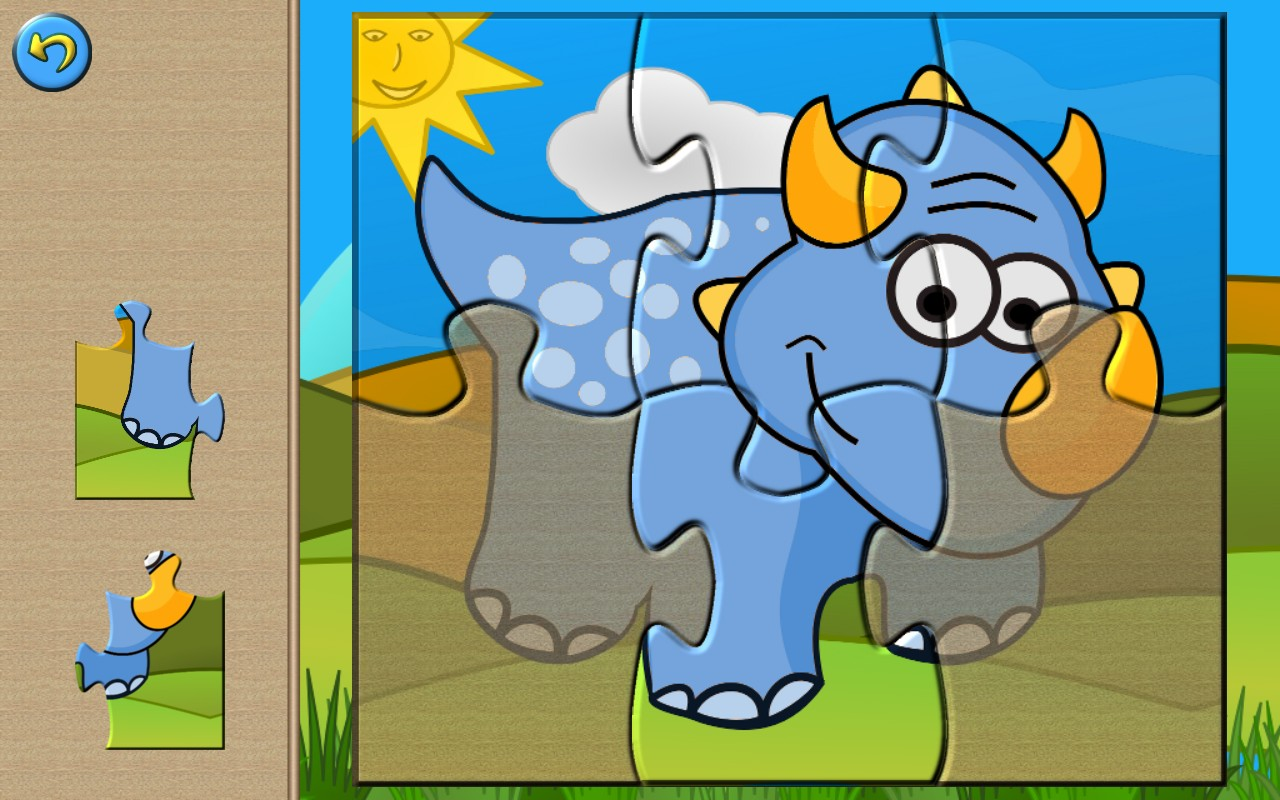
\includegraphics[width=\linewidth]{./Figures/chapter-01/baby-01.jpg}
	%		
\includegraphics[width=\linewidth,height=\textheight]{./Figures/chapter-01/baby-02.jpg}
	%	\caption{}
\end{figure}
\end{frame}


%%%%%%%%%%%%%%%%%%%%%%%%%%%%%%%%%%%%%%%%%%%%%%%%%%%%%%
\begin{frame}
\frametitle{Transnational DB Use cases}
\begin{figure}[ht]

\centering
%	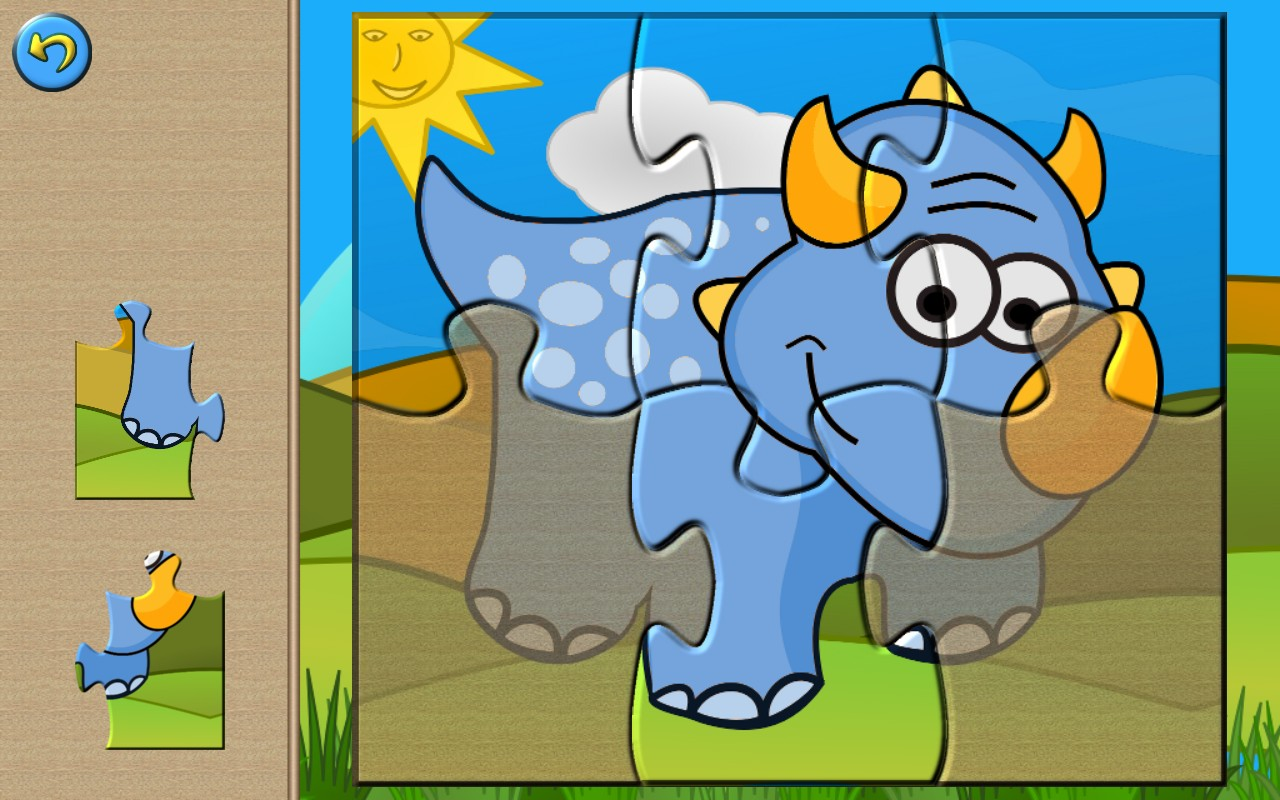
\includegraphics[width=\linewidth]{./Figures/chapter-01/baby-01.jpg}

\includegraphics[width=\linewidth]{./Figures/chapter-01/baby-02.jpg}
%	\caption{}
\end{figure}
\end{frame}


%%%%%%%%%%%%%%%%%%%%%%%%%%%%%%%%%%%%%%%%%%%%%%%%%%%%%%
\begin{frame}
\frametitle{DWH Use cases}
\begin{figure}[ht]

\centering

\includegraphics[width=\linewidth,height=.8\textheight]{./Figures/chapter-01/Marvel-03.jpg}
%	\caption{}
\end{figure}
\end{frame}

%%%%%%%%%%%%%%%%%%%%%%%%%%%%%%%%%%%%%%%%%%%%%%%%%%%%%%
\begin{frame}
\frametitle{DWH Use cases}
\begin{figure}[ht]

\centering
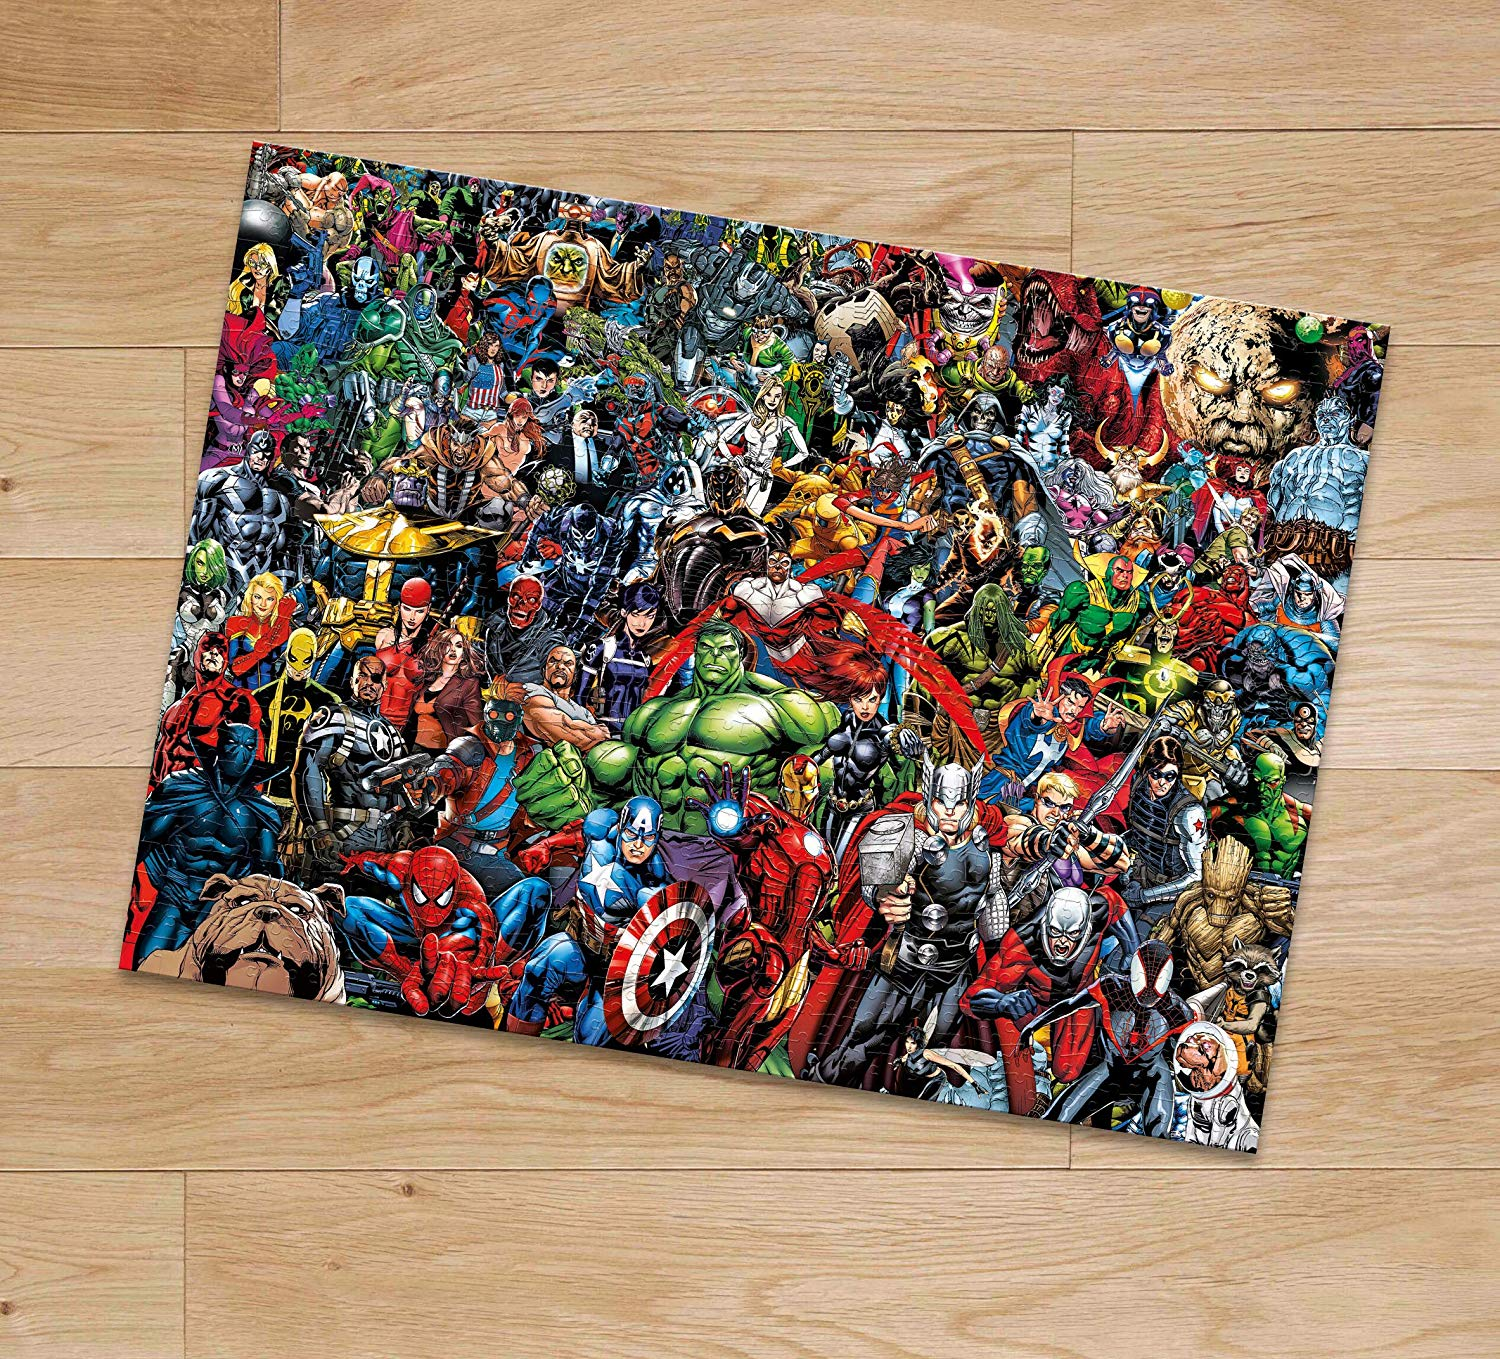
\includegraphics[width=\linewidth,height=.8\textheight]{./Figures/chapter-01/Marvel-02.jpg}
%	\caption{}
\end{figure}
\end{frame}

%%%%%%%%%%%%%%%%%%%%%%%%%%%%%%%%%%%%%%%%%%%%%%%%%%%%%%
\begin{frame}
\frametitle{DWH Use cases}
\begin{figure}[ht]

\centering
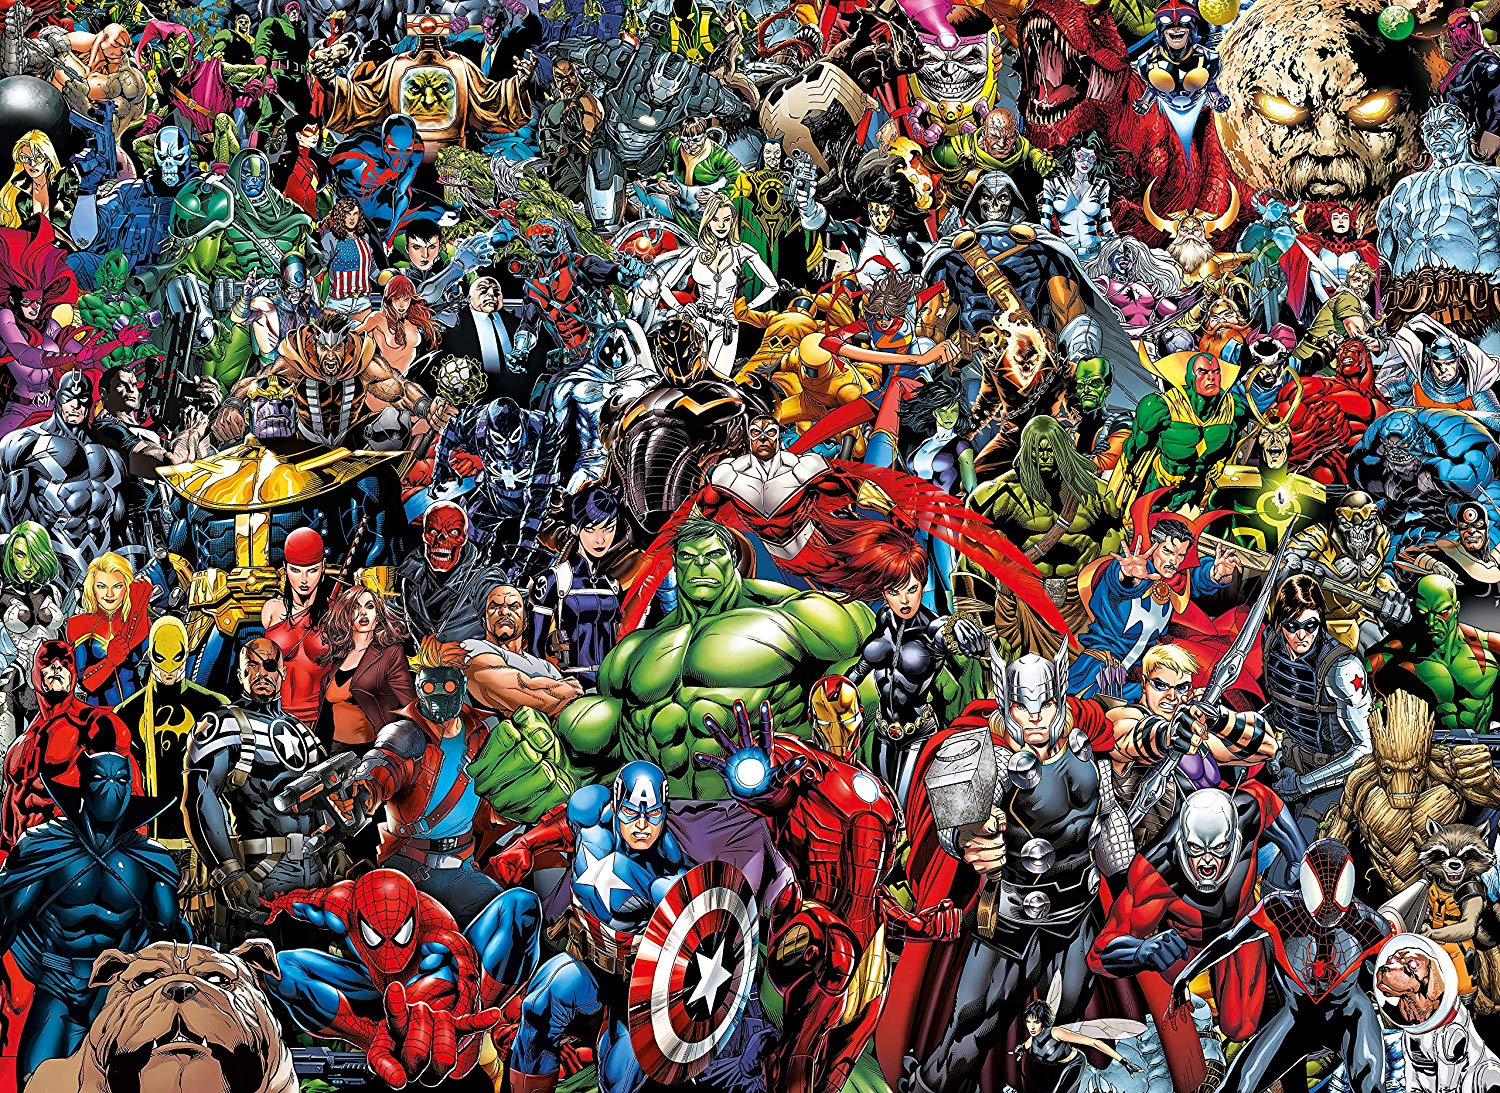
\includegraphics[width=\linewidth,height=.8\textheight]{./Figures/chapter-01/Marvel-01.jpg}
%	\caption{}
\end{figure}
\end{frame}
%%%%%%%%%%%%%%%%%%%%%%%%%%%%%%%%%%%%%%%%%%%%%%%%%%%%%%


%%%%%%%%%%%%%%%%%%%%%%%%%%%%%%%%%%%%%%%%%%%%%%%%%%%%%%
\subsubsection{Types of DWH}
\begin{frame}
\frametitle{Motivation to Data Warehouse}
Types of Data Warehouse
\begin{description}
\item [\textbf{Enterprise Data Warehouse (EDWH)}] It provides decision support service across the enterprise. It offers a unified approach for organizing and representing data (DWH Model). It offers data classifications according to the subject with privileges policy.
\item [\textbf{Operational Data Store (ODS):}] is a central database that provides an up-to-date (real-time) data from multiple transnational systems for operational reporting into a single DWH.

%% for real time questions and answers. call ODS using intermidiate data store. DWH is day -1 (billing & subscribtions). Oracle (Loading or headache) && CDC capture change interest column not row
\item [\textbf{Data Mart:}] A data mart is a subset of the data warehouse. It specially designed for a particular line of business, such as sales, finance, sales or finance. In an independent data mart, data can collect directly from sources.
\end{description}

\end{frame}

%%%%%%%%%%%%%%%%%%%%%%%%%%%%%%%%%%%%%%%%%%%%%%%%%%%%%%

\begin{frame}
\frametitle{DWH vs ODS vs Data Mart}


\begin{table}[t]
\centering	
\resizebox{\columnwidth}{!}{%

%		\centering
\begin{tabular}{|c | c | c| c |}
\hline
\textbf{Metric}  & \textbf{DWH}& \textbf{ODS} & \textbf{Data Mart} \\
\hline
Latency & Day -1  & Real-time & Day -1 \\			
Data level  & Transnational & Transnational & Summary \\
Historical  & Long-term & Snapshot & Aggregated Long-Term \\
Size & TB/PB & GB & GB/TB\\
Orientation & Multi sources & Multi sources & Product\\
Business Units & Multi organizational units & Product team & Business team \\
\hline
\end{tabular}
%		\caption{Data Representation Combination Matrix}\label{Tab:Data_Representation_Matrix}
}
\end{table}
\end{frame}


%%%%%%%%%%%%%%%%%%%%%%%%%%%%%%%%%%%%%%%%%%%%%%%%%%%%%%%%%%%%%%%%%%%%%%%%
\subsubsection{Use Cases of Operational DB vs DWH}

\begin{frame}
\frametitle{Use case (Operational DB)}

\begin{itemize}[<+->]

\item A telecommunication company named \textbf{XTec}.
\newline
\item They have lots of systems. One of this systems is a CRM system as example of operational DB.
\begin{itemize}[<+->]

\item The CRM system handles the customer activities with the company including (sales, change in customer plans, and other activities).
\item This system has a backend database (MySQL).
\item CRM team can report their sales and customer activities from their database.
\item Product owner can take a decision based on their system backend reports.

\end{itemize}

\end{itemize}

\end{frame}

%%%%%%%%%%%%%%%%%%%%%%%%%%%%%%%%%%%%%%%%%%%%%%%%%%%%%%

\begin{frame}
\frametitle{Use case (DWH)}

\begin{itemize}[<+->]

\item What is the need for DWH?		
\begin{itemize}[<+->]
\item This company has other systems for example: billing, charging, signaling.	
\item They need to report information related to the CRM, billing, and signaling source systems in one report.
\item So, they need to ingest (transfer) the data from the source systems to one single database.
\item The decision from the DHW is a \textbf{global and strategical decision.}
\item If the company needs to build a machine learning model which needs data from different sources. They need to load the data from a centralized database rather than read each source alone.
\end{itemize}

\end{itemize}

\end{frame}
%%%%%%%%%%%%%%%%%%%%%%%%%%%%%%%%%%%%%%%%%%%%%%%%%%%%%%


\begin{frame}
\frametitle{Use case (DWH)}
\centering
The Full picture required a DWH. However, we still need the other operational databases for product development perspective.


\end{frame}
%%%%%%%%%%%%%%%%%%%%%%%%%%%%%%%%%%%%%%%%%%%%%%%%%%%%%%

\begin{frame}
\frametitle{Use case (ODS)}
\centering

\begin{itemize}[<+->]
\item Why do we need the ODS?
\item 	How does it fit in our system?
\end{itemize}


\end{frame}
%%%%%%%%%%%%%%%%%%%%%%%%%%%%%%%%%%%%%%%%%%%%%%%%%%%%%%


%%%%%%%%%%%%%%%%%%%%%%%%%%%%%%%%%%%%%%%%%%%%%%%%%%%%%%

\begin{frame}
\frametitle{Use case (ODS)}
\centering
\textbf{XTec} has a call center system which handles the customer inquiries. This system requires the some data related to usage, customer information, billing details to be calculated and accumulated in \textbf{real-time} to be able to give the customer the right answer for his inquires.

\end{frame}
%%%%%%%%%%%%%%%%%%%%%%%%%%%%%%%%%%%%%%%%%%%%%%%%%%%%%%
%%%%%%%%%%%%%%%%%%%%%%%%%%%%%%%%%%%%%%%%%%%%%%%%%%%%%%
\begin{frame}
\frametitle{Use case (ODS)}

	\begin{itemize}[<+->]
		\item So, What is the challenge for this system?
			\begin{itemize}[<+->]		
				\item It needs specific information from different source systems.
				\item It requires to track the source system database changes or update in real-time.
				\item It's functionality is based on the aggregate data not the transactions for example (It needs the total outgoing calls till time or it needs the total charging amounts from prepaid or the available limits from billing if it is postpaid).
			\end{itemize}
	\end{itemize}

\end{frame}
%%%%%%%%%%%%%%%%%%%%%%%%%%%%%%%%%%%%%%%%%%%%%%%%%%%%%%
\begin{frame}
\frametitle{Use case (ODS)}

	\begin{itemize}[<+->]
		\item ODS is based on change data capture (CDC). This approach used to determine the data change and apply action based on this change.
		\item ODS uses the real-time aggregations to support the online systems from different source systems.
	\end{itemize}
\end{frame}
%%%%%%%%%%%%%%%%%%%%%%%%%%%%%%%%%%%%%%%%%%%%%%%%%%%%%%
\subsection{DWH Characteristics}
\begin{frame}
\frametitle{DWH Characteristics}
%these is not a definitions, we just show the meaning and the understanding.
\begin{wideitemize}
\item The characteristics of DWH:
	\begin{wideitemize}
		\item Integrated: \textit{DWH is an integrated environment which allows us to integrate different source systems. Data are modeled (organized) into a unified manner.} %regardless of the original source
	
		\item Time-Variant: \textit{Data modeled (organized) based on time periods (hourly, daily, weekly, monthly, quarterly, yearly, etc.)}
	
		\item Subject-oriented: \textit{DWH main target is to support business needs for the whole organization including (decision makers, departments, and specific user requirements)}.
	
		\item Non-Volatile: \textit{It refers to the data will not erased or deleted (It could be archived and retrieved when needed). Data can be accumulated daily the new snapshots (refreshed at based on the source system interval. For example, It could be updated daily, weekly, and monthly).}
	\end{wideitemize}	
\end{wideitemize}
%https://www.guru99.com/data-warehouse-architecture.html

\end{frame}
%%%%%%%%%%%%%%%%%%%%%%%%%%%%%%%%%%%%%%%%%%%%%%%%%%%%%%
\subsection{Data Warehouse Architecture}
%%%%%%%%%%%%%%%%%%%%%%%%%%%%%%%%%%%%%%%%%%%%%%%%%%%%%%
\begin{frame}
\frametitle{DWH Architecture Overview}


\end{frame}


%%%%%%%%%%%%%%%%%%%%%%%%%%%%%%%%%%%%%%%%%%%%%%%%%%%%%%
\begin{frame}
\frametitle{DWH Architecture Overview}
\begin{figure}[ht]
	
	\centering
	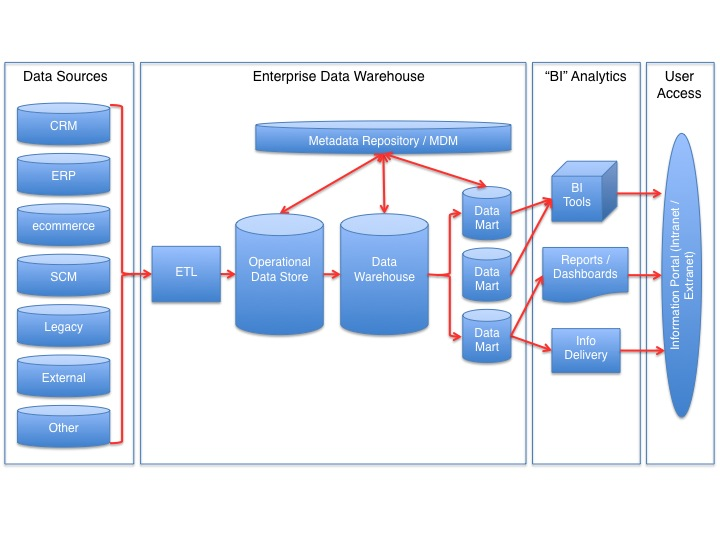
\includegraphics[width=.9\linewidth,height=.8\textheight]{./Figures/chapter-01/Datawarehouse_reference_architecture.jpg}
	%https://commons.wikimedia.org/wiki/File:Datawarehouse_reference_architecture.jpg
	%		
\includegraphics[width=\linewidth,height=\textheight]{./Figures/chapter-01/baby-02.jpg}
	\caption{taken from XXXX}
\end{figure}
\end{frame}


%%%%%%%%%%%%%%%%%%%%%%%%%%%%%%%%%%%%%%%%%%%%%%%%%%%%%%
\subsubsection{ETL Process}
%%%%%%%%%%%%%%%%%%%%%%%%%%%%%%%%%%%%%%%%%%%%%%%%%%%%%%
\subsubsection{ETL vs ELT When? Why?}

%%%%%%%%%%%%%%%%%%%%%%%%%%%%%%%%%%%%%%%%%%%%%%%%%%%%%%
\subsection{Data Models}
\begin{frame}
\frametitle{What is data model?}
Data model is
\begin{itemize}[<+->]
	\item An abstract model that organizes elements of data.
	\item It describes the objects, entities and data structure properties, semantic, and constraint.
	\item It formalizes the relationship between entities.
	\item It describes how application (report) API data manipulation.
	\item It describes the conceptual design of a business or an application with its flow, logic, semantic information (rules), and how things are done.
	\item It refers to a set of concepts used in defining such as entities, attributes, relations, or tables.
\end{itemize}
\end{frame}

%%%%%%%%%%%%%%%%%%%%%%%%%%%%%%%%%%%%%%%%%%%%%%%%%%%%%%
\begin{frame}
\frametitle{What is data model?}

Data model is not	
\begin{itemize}
	\item a science.
	\item a static design for each organization.
	\item a type of database.
	\item a new invention which needs to be done for each project.
\end{itemize}


Data model is		
\begin{itemize}
	\item an engineering design practices.
	\item a general concepts which lead to build full architecture.
	\item different based on the use case and the database type.
	\item customizable and we can utilize some of ready built architecture. 
	\item implementing using different ways.
	\item affecting the information reporting performance and ways.
\end{itemize}

\end{frame}
%%%%%%%%%%%%%%%%%%%%%%%%%%%%%%%%%%%%%%%%%%%%%%%%%%%%%%

\begin{frame}
\frametitle{Why does data models are important?}
\begin{wideitemize}	
	\item Data models are currently affecting software design. 
	\item It decides how engineers will think about the problem they are solving.
\end{wideitemize}
\end{frame}
%%%%%%%%%%%%%%%%%%%%%%%%%%%%%%%%%%%%%%%%%%%%%%%%%%%%%%
\subsubsection{Data Model Design}
\begin{frame}
\frametitle{Data Model Design vs Implementation}
\begin{itemize}[<+->]
	\item You need to build a home. So, how do we design this home?
		\begin{itemize}[<+->]
			\item Determine if the home is one level or multi-level and decide man bedrooms and bathrooms for each floor. (User needs)
			\item Hire an architect to put the architecture in more detailed way for example, the size for each room, the distribution of the wireds, where the plumbing fixtures will be placed, etc. (Architecture phase)
			\item Decide the decorations, colors for each room, carpets, etc. 
		\end{itemize}
	\item What do we do for the implementation?
		\begin{itemize}[<+->]
			\item Hire a contractor to build (implement the design) the home. 
			\item This phase will implement the design but it also include some detail related to the actual way to build the tools and the material. (Physical Design)
		\end{itemize}		
\end{itemize}
\end{frame}


%%%%%%%%%%%%%%%%%%%%%%%%%%%%%%%%%%%%%%%%%%%%%%%%%%%%%%%%
\begin{frame}
\frametitle{DWH Architecture Overview}
There are mainly three types of Datawarehouse Architectures: -
%https://www.guru99.com/data-warehouse-architecture.html
\begin{wideitemize}
	\item Single-tier architecture.
	\item Two-tier architecture.
	\item Three-tier architecture.
\end{wideitemize}

\end{frame}

%%%%%%%%%%%%%%%%%%%%%%%%%%%%%%%%%%%%%%%%%%%%%%%%%%%%%%
\subsubsection{File Formats}

\begin{frame}
\frametitle{\subsecname}
\begin{itemize}[<+->]
	\item Any Big Data solution working based distributed systems.
	\item What is distributed systems in brief?
\end{itemize}
\end{frame}
%%%%%%%%%%%%%%%%%%%%%%%%%%%%%%%%%%%%%%%%%%%%%%%%%%%%%%
\subsubsection{Data Encoding and Formats}

\begin{frame}
\frametitle{\subsecname}
\begin{itemize}[<+->]
	\item Any Big Data solution working based distributed systems.
	\item What is distributed systems in brief?
\end{itemize}
\end{frame}
%%%%%%%%%%%%%%%%%%%%%%%%%%%%%%%%%%%%%%%%%%%%%%%%%%%%%%
\subsubsection{Data Compression Technique}

\begin{frame}
\frametitle{\subsecname}
\begin{itemize}[<+->]
\item Any Big Data solution working based distributed systems.
\item What is distributed systems in brief?
\end{itemize}
\end{frame}
%%%%%%%%%%%%%%%%%%%%%%%%%%%%%%%%%%%%%%%%%%%%%%%%%%%%%%%%%%%%%%%%%%%%%%%%%%%

\subsubsection{Data Archiving and Retention}
\begin{frame}
\frametitle{\subsecname}
\begin{itemize}[<+->]
	\item some details about hot vs cold storage,
\end{itemize}
\end{frame}
%%%%%%%%%%%%%%%%%%%%%%%%%%%%%%%%%%%%%%%%%%%%%%%%%%%%%%%%%%%%%%%%%%%%%%%%%%%

%%%%%%%%%%%%%%%%%%%%%%%%%%%%%%%%%%%%%%%%%%%%%%%%%%%%%%%%
\subsubsection{Different Types of Storage}
\begin{frame}

\frametitle{Cold storage vs Hot storage}

some details about hot vs cold storage,

\end{frame}
%%%%%%%%%%%%%%%%%%%%%%%%%%%%%%%%%%%%%%%%%%%%%%%%%%%%%%

\subsection{DWH On Cloud}



\subsection{Further Readings and Assignment}


%%%%%%%%%%%%%%%%%%%%%%%%%%%%%%%%%%%%%%%%%%%%%%%%%%%%%%%%%%%%%%%%%%%%%%%%%%%
%%% Local Variables:
%%% mode: latex
%%% TeX-master: "../main"
%%% TeX-engine: xetex
%%% End:
